\section{Problem 1}

\subsection{Question}
\vspace*{10pt}
Demonstrate that you know how to use \enquote{curl} well enough to
correctly POST data to a form.  Show that the HTML response that
is returned is \enquote{correct}.  That is, the server should take the
arguments you POSTed and build a response accordingly.  Save the
HTML response to a file and then view that file in a browser and
take a screen shot.
\vspace*{5mm}
\subsection{Answer}
\vspace{1mm}
The \textit{cURL} command is a handy command-line utility for making HTTP requests. Using \textit{curl} to stream data, it can be a very useful troubleshooting tool. It also allows us to assess \enquote{raw} streaming performance. The following command \textit{(See Figure: 1)}  will get the content of the URL and display it in the terminal. 
\\
\\
\textbf{Make requests with data:} 
\\
I have created a simple php page $curl\_posted.php$, which accepts two arguments:
\vspace*{1mm}
\begin{center}
	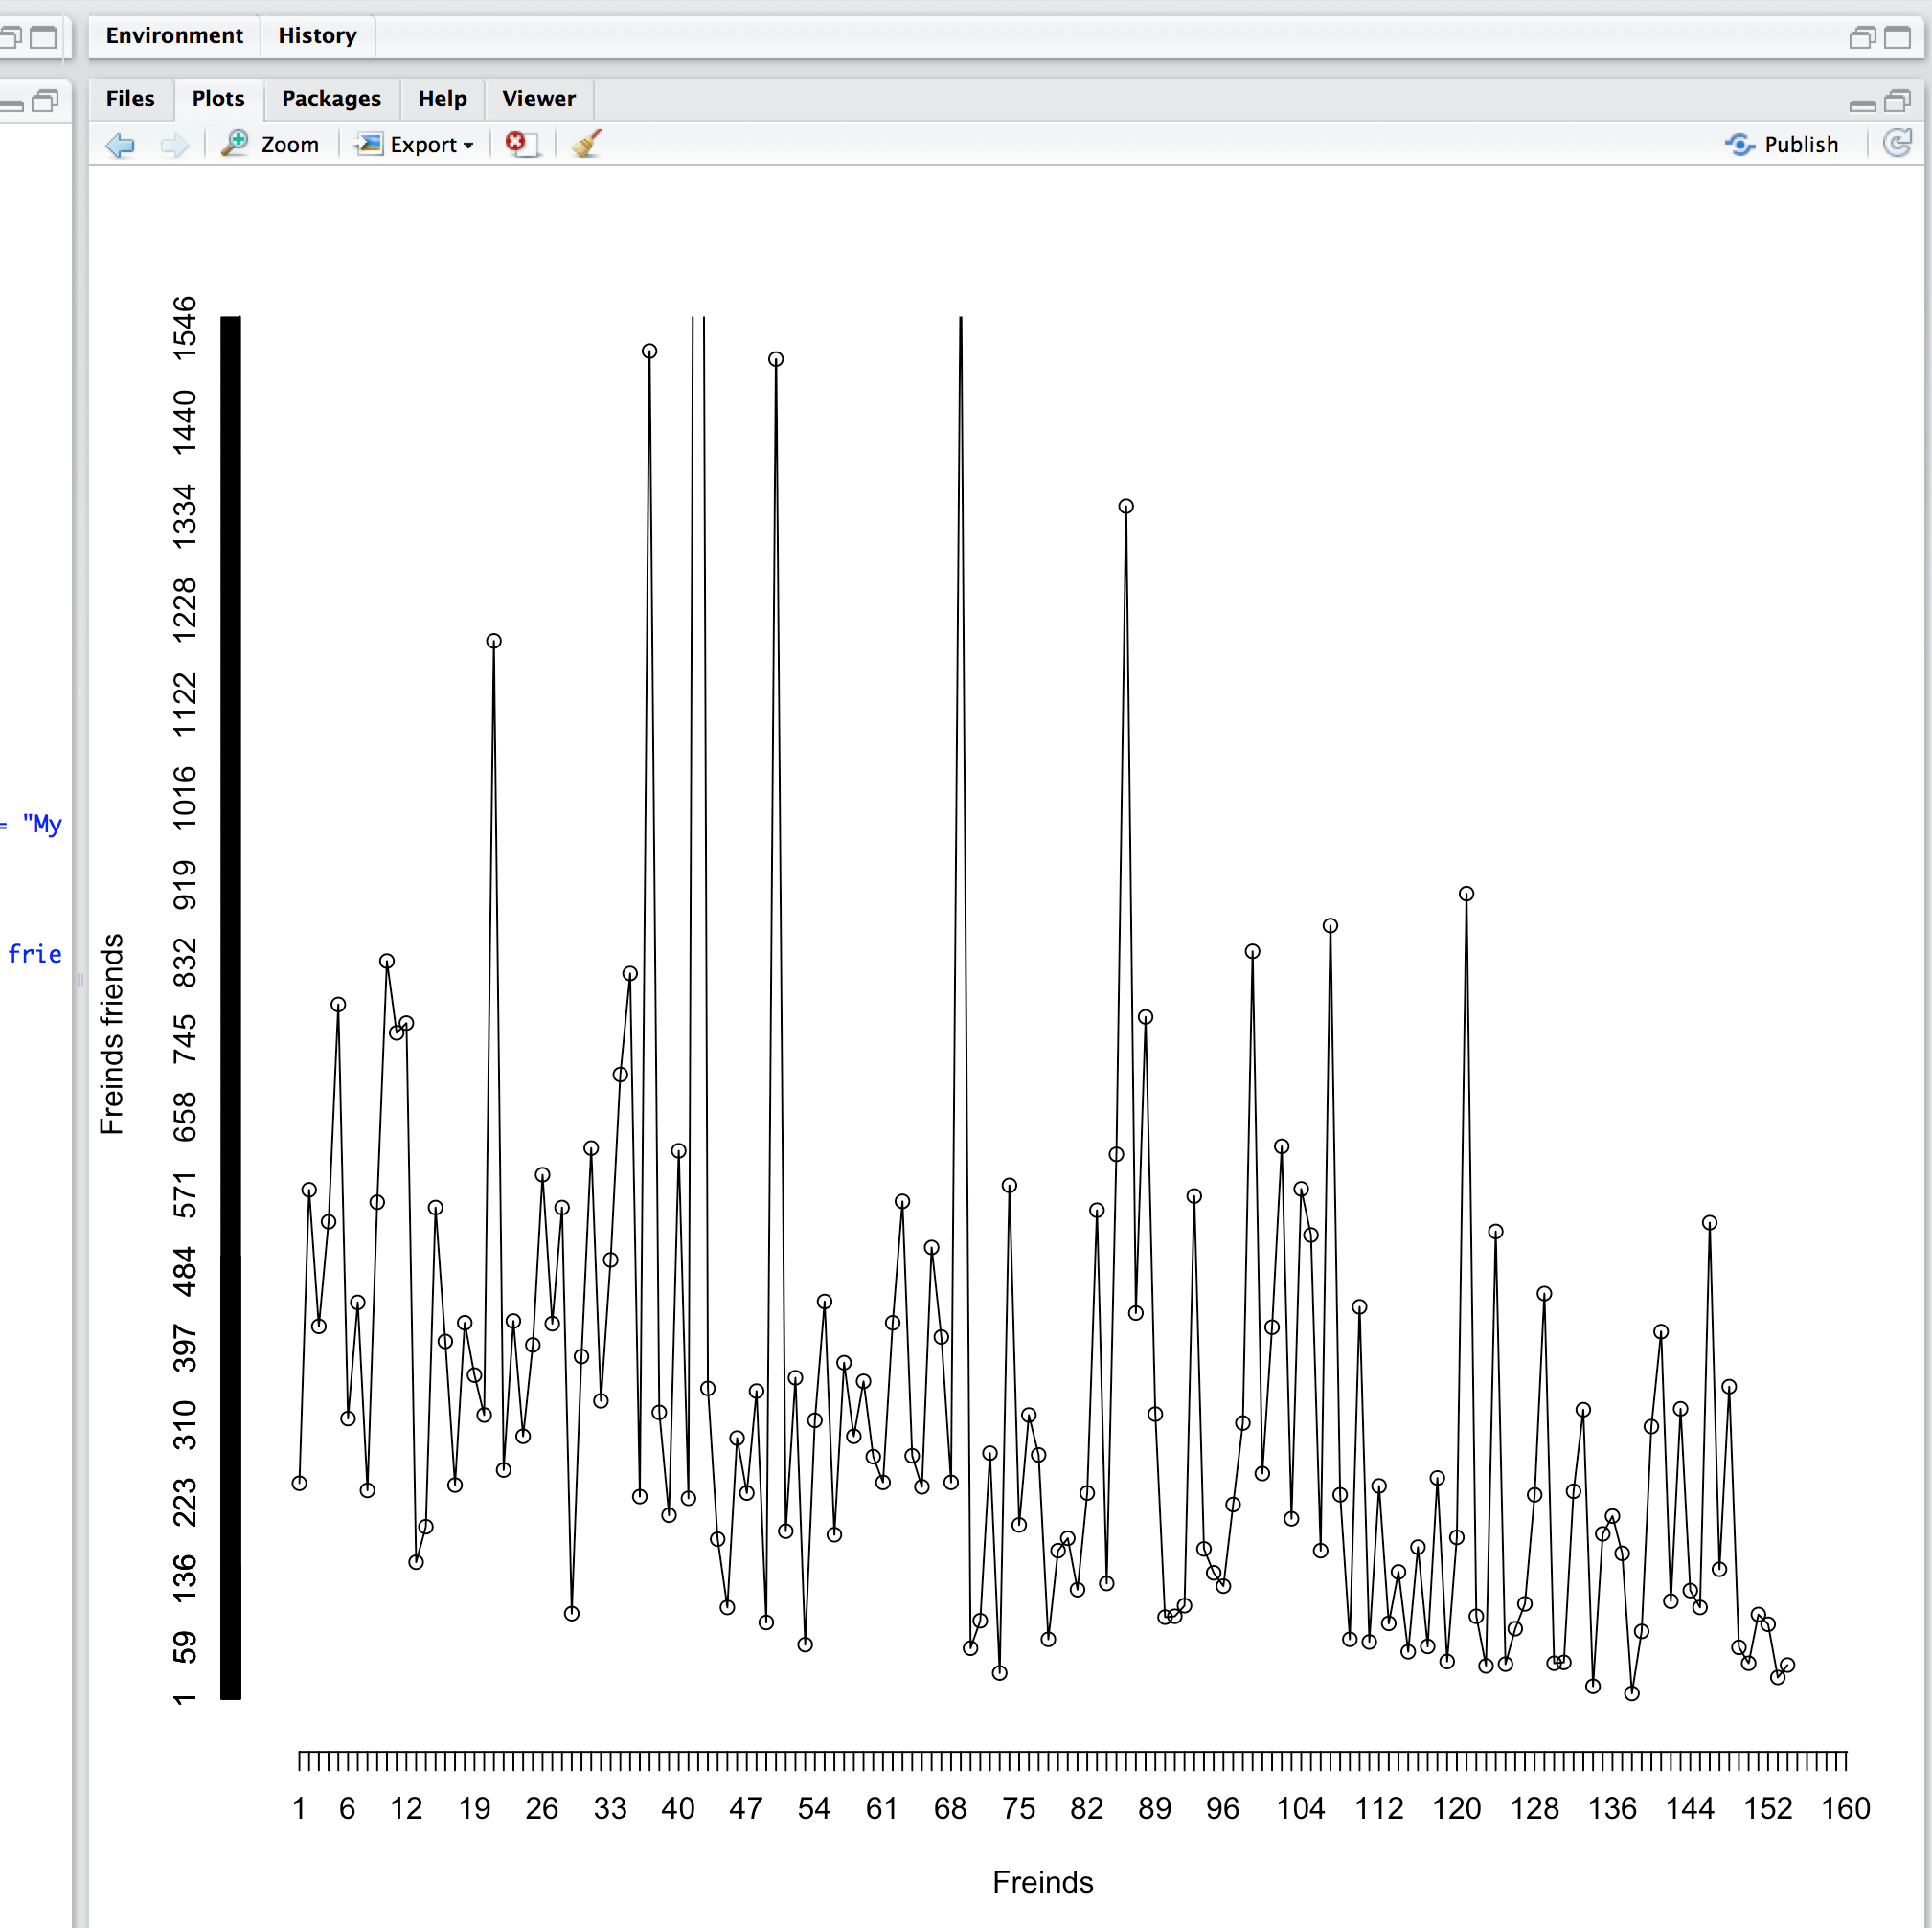
\includegraphics[scale=.75]{Q1/fig1.png}\\
	\textit{Figure 1: Screen shot of using curl Command}
\end{center}
\vspace*{5mm}
If there's a \enquote{normal} post, use -d to post. 
-d takes a full \enquote{post string}, which is in the format\\
\centerline{$<variable1>=<data1>\&<variable2>=<data2>\&...$}
The \enquote{variable} names are the \enquote{names} set with "firstname=" in the $<input>$ tags, and the data is the contents you want to fill in for the inputs. The data \textbf{must} be properly URL encoded. 
\\
\\
We can save the result of the curl command to a file by using -o/-O options.
\begin{itemize}
	\item{-o (lowercase o): result will be saved in the filename provided in the command line}
	\item{-O (uppercase O): filename in the URL will be taken and it will be used as the filename to store the result}
\end{itemize}
 To store the output in a file\textit{(See Figure: 5)}, redirect it as shown above. This will also display some additional download statistics \textit{(See Figure: 4.)}. 

\newpage
\begin{lstlisting}[frame=single,numbers=left]
<!DOCTYPE html PUBLIC "-//W3C//DTD XHTML 1.0 Transitional//EN"
  "http://www.w3.org/TR/xhtml1/DTD/xhtml1-transitional.dtd">
<html xmlns="http://www.w3.org/1999/xhtml"><head>
 4 <meta http-equiv="Content-Type" content="text/html;
  charset=utf-8" />
<title>CS532 Web Science | Assignment 1</title>
</head>
<body>
<body>
<form method="POST" action="curl_posted2.php">
First name: <input type="text" name="firstname"><br>
Last name: <input type="text" name="lastname"><br>
<input type="submit" name="press" value="OK">
</form>
</body>
</html>
\end{lstlisting}
\centerline{\textbf{$curl\_posted.php$}}
\vspace{10pt}
\begin{center}
	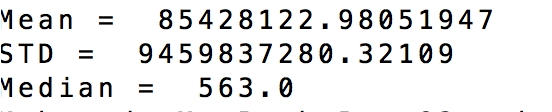
\includegraphics[scale=1.375]{Q1/fig2.png}\\
	\centerline{\textit{Figure 2: Screen shot of $curl\_posted.php$ page}}
\end{center}



\newpage
\vspace*{10pt}
Following php script is executed at the server side, when the form is submitted: 
\vspace*{1mm}
\begin{lstlisting}[frame=single,numbers=left]
<!DOCTYPE html PUBLIC "-//W3C//DTD XHTML 1.0 Transitional//EN"
"http://www.w3.org/TR/xhtml1/DTD/xhtml1-transitional.dtd">
<html xmlns="http://www.w3.org/1999/xhtml">
<head>
<meta http-equiv="Content-Type" content="text/html; 
 charset=utf-8" />
<title>CS532 Web Science | Assignment 1</title>
</head>
<body>
<?php
	$firstname = $_POST['firstname'];
	$lastname = $_POST['lastname'];
 echo '\n<h2> Your Full Name is'." ".$firstname." 
".$lastname." ".'</h2>';
?>
</body>
</html>
\end{lstlisting}
\centerline{\textbf{$curl\_posted2.php$}}
\vspace*{5pt}
\begin{center}
	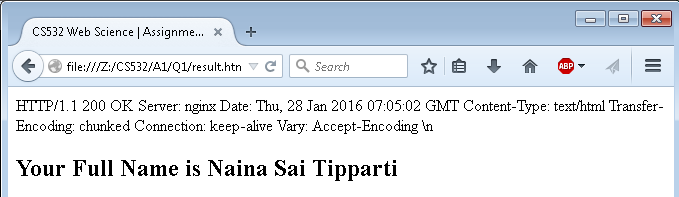
\includegraphics[scale=.975]{Q1/fig4.png}\\
	\centerline{\textit{Figure 3: Screen shot of saved HTML response}}
\end{center}

\newpage
\vspace*{5pt}
If curl fails where it isn't supposed to, if the servers don't let you in,
if you can't understand the responses: use the -v flag \textit{(See Figure: 3)} to get verbose
  fetching. Curl will output lots of info and what it sends and receives in
  order to let the user see all client-server interaction (but it won't show
  you the actual data).\\
  \\
\begin{center}
	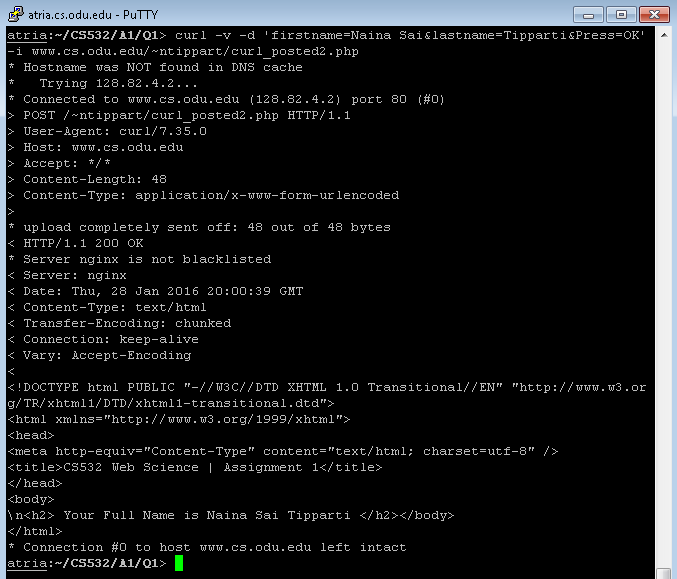
\includegraphics[scale=0.85]{Q1/fig5.png}
	\centerline{\textit{Figure 4: Screen short of HTML Response}}
\end{center}
\begin{center}
	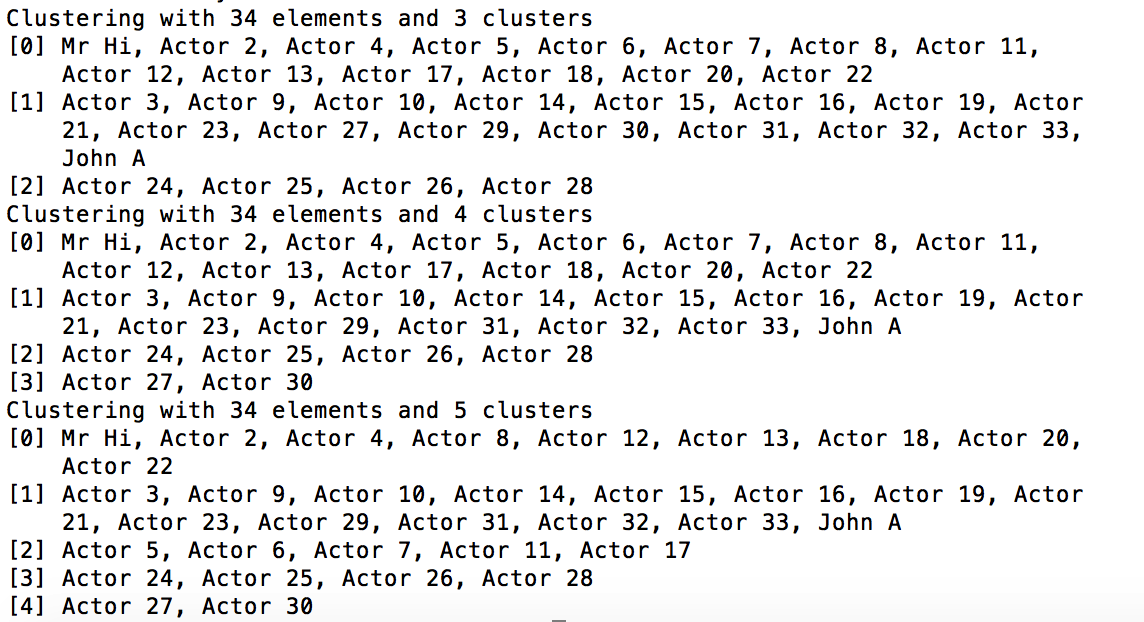
\includegraphics[scale=0.85]{Q1/fig3.png}\\
	\centerline{\textit{Figure 5: Screen shot of curl POST}}
\end{center}
\vspace*{5mm}


   
